\subsection{Borehole examples}
The next example is based on synthetic borehole DC data, where the simulated data are
%
\begin{enumerate}
\item Surface data simulated using dipole-dipole configuration
\item Borehole data simulated using larger dipole with one transmitter electrode placed in the borehole
\item Combination of surface and borehole data simulation
\end{enumerate}
The synthetic data were generated using a 2D model (Figure \ref{fig:boreholeSyn}) that contains a 25-m thick overburden of 100 Ohm-m over a 1000 Ohm-m half space. A 1 Ohm-m prism is located buried so that its top is 100 m below the surface. The prism is 100 m $\times$ 100 m. The model was discretized onto a 6869 cell mesh (104 horizontal by 66 vertical cells. Smallest cell equals 10 m by 5 m). The locations of two boreholes are also shown in the figure.
%
\begin{figure}
\centering
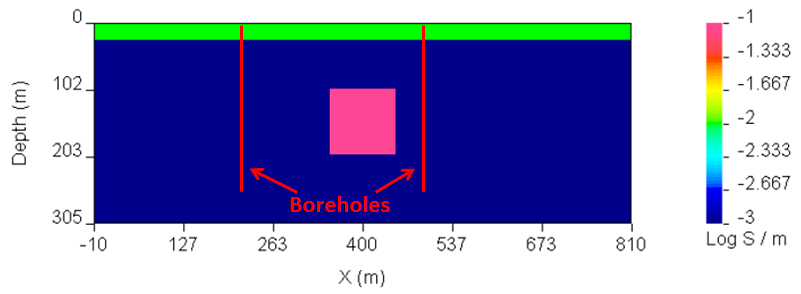
\includegraphics[width=0.5\columnwidth]{boreholeSyn}
\caption{The synthetic model used for the three borehole examples.}
\label{fig:boreholeSyn}
\end{figure}

The first synthetic data set is surface-only dipole-dipole array. Electrodes are located every 25 m within the region (0 m, 800 m) and each dipole-dipole survey used n=1,15. A total of 30 transmitter locations were used. The total number of data is 345. The data were contaminated with 5\% Gaussian noise and inverted with a chi factor of 1 (see control input file configuration provided below). The inversion has converged in 14 iterations. The results of the inversion of surface data are presented in Figure \ref{fig:synBsurf}.
%
\begin{fileExample}
\begin{tabular}{|ll|}
\hline
OBS LOC\_XZ dc\_surface.dat & ! General-formatted DC data \\
MESH FILE mesh2d.msh & ! Mesh \\
INVMODE CG & ! Use CG \\
REF\_MOD FILE 1e-3 & ! Reference model \\
\hline
\end{tabular}
\end{fileExample}
%
\begin{figure}
\centering
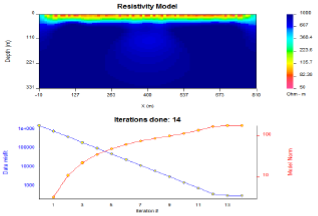
\includegraphics[width=0.5\columnwidth]{bSurf}
\caption{(a) The recovered model from the inversion of synthetic surface data set and (b) the associated convergence curves.}
\label{fig:synBsurf}
\end{figure}

Next the same conductivity model was used to simulate a synthetic borehole data set for two boreholes located at $x=200$ and $x=500$. Electrodes were spaced every 25 m down each borehole to a maximum depth of 250 m. The transmitter electrodes are located in the opposite boreholes in all possible configurations. The schematic diagram illustrating this survey configuration is shown in Figure \ref{fig:bSchem}. This resulted in a total of 121 transmitters. Each transmitter configuration is a common-current source for up to 20 receiver dipoles in both boreholes. The total number of data is 2200. The simulated data set was contaminated by 5\% Gaussian noise and inverted using same inversion parameters as the surface data set. The results are shown in Figure \ref{fig:bCurr}.
%
\begin{figure}
\centering
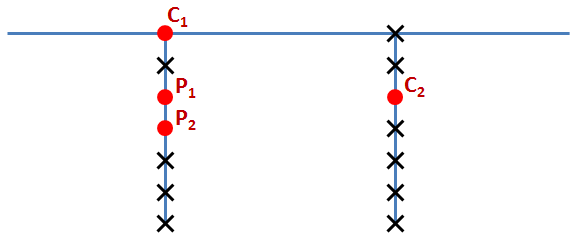
\includegraphics[width=0.5\columnwidth]{bSchem}
\caption{A schematic of the survey configuration for the synthetic borehole example. Red dots mark the electrode positions.}
\label{fig:bSchem}
\end{figure}
%
\begin{figure}
\centering
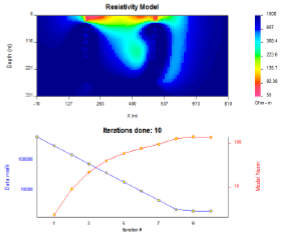
\includegraphics[width=0.5\columnwidth]{bCurr}
\caption{(a) The recovered model from the inversion of synthetic down-hole data set and (b) the associated convergence curves.}
\label{fig:bCurr}
\end{figure}

Further, the data sets were combined to accommodate 151 transmitter locations and 2545 data. The combined data set was inverted with the same parameters as each individual data set with the results shown in Figure \ref{fig:bAll}. As it is evident from these three inversions, the surface geometry alone has strong limitations in depth resolution, while the borehole configuration has limitations in near-surface recovery and it is the combination of the two surveys, which allows better recovery of the conductivity.
%
\begin{figure}
\centering
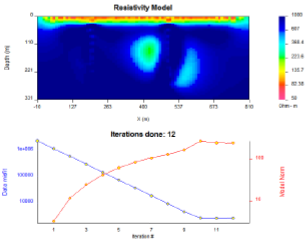
\includegraphics[width=0.5\columnwidth]{bAll}
\caption{(a) The recovered model from the inversion of synthetic down-hole and surface data sets and (b) the associated convergence curves.}
\label{fig:bAll}
\end{figure}

The inversion was then constrained using a weighting matrix with small weights for the vertical interface at the depth of 25 m, ensuring a sharper contrast across this boundary and large weights assigned to all horizontal interfaces up to the depth of 25 m, ensuring a smooth transition of electrical properties in this direction. This weighting matrix is designed, assuming there is prior knowledge about the overburden and defines the latter as a horizontal (laterally smooth) structure with abrupt transition in the vertical direction. The control file used for this inversion is shown below. The result of the inversion is shown in Figure \ref{fig:bAllWght}.
%
\begin{fileExample}
\begin{tabular}{|ll|}
\hline
OBS LOC\_XZ obs\_dc\_n.dat & ! General-formatted DC data \\
MESH FILE mesh2d.msh & ! Mesh \\
INVMODE CG & ! Use CG \\
REF\_MOD FILE 1e-3 & ! Reference model \\
WEIGHT FILE weights.txt & ! Weight file \\
\hline
\end{tabular}
\end{fileExample}
%
It is evident from Figure \ref{fig:bAllWght}, that not only did the weighting function assure clean resolution of overburden, but it also helped to remove some noise from the background, if compared with Figure \ref{fig:bAll}.
%
\begin{figure}
\centering
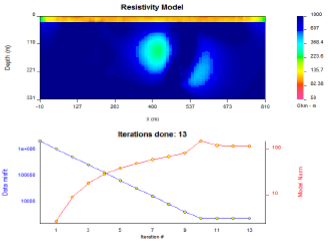
\includegraphics[width=0.5\columnwidth]{bAllWght}
\caption{(a) The recovered model from the inversion of synthetic down-hole and surface data sets with a weighting constraint and (b) the associated convergence curves.}
\label{fig:bAllWght}
\end{figure}

The next step was to simulate a scenario, when the down-hole conductivity data is available. This was done using the inactive cells constraint. Figure \ref{fig:bAllAct}a shows the new reference model with fixed cells along $x=200$ and $x=500$ to the depth of 250 m. The data were inverted using inactive cells constraint with no ability to affect the neighbouring cells (Figure \ref{fig:bAllAct}b), with ability to interfere with the neighbours (Figure \ref{fig:bAllAct}c) and in combination with the weighting matrix (Figure \ref{fig:bAllAct}d).
%
\begin{fileExample}
\begin{tabular}{|ll|}
\hline
OBS LOC\_XZ obs\_dc\_n.dat & ! General-formatted DC data \\
MESH FILE mesh2d.msh & ! Mesh \\
INVMODE CG & ! Use CG \\
REF\_MOD FILE 1e-3 & ! Reference model \\
ACTIVE\_CELLS active.txt & ! Active cell file \\
\hline
\end{tabular}
\end{fileExample}
%
Finally, the area of inactive cells was extended, simulating a scenario, when a-priori information suggests that the anomalous conductivity lies between the two boreholes. The final control file used for inverting data under these constraints is presented below:
%
\begin{fileExample}
\begin{tabular}{|ll|}
\hline
OBS LOC\_XZ obs\_dc\_n.dat & ! General-formatted DC data \\
MESH FILE mesh2d.msh & ! Mesh \\
INVMODE CG & ! Use CG \\
REF\_MOD FILE 1e-3 & ! Reference model \\
WEIGHT FILE weights.txt & ! Weight file \\
ACTIVE\_CELLS active.txt & ! Active cell file \\
\hline
\end{tabular}
\end{fileExample}
%
The results of the final inversion are presented in Figure \ref{fig:bAllWghtAct}.

%
\begin{figure}
\centering
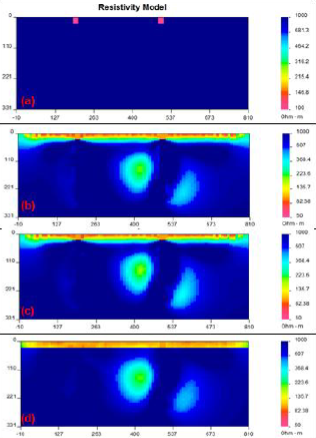
\includegraphics[width=0.5\columnwidth]{bAllAct}
\caption{(a) The new reference model, accommodating the active cells. The inversion was then carried out such that the inactive cells both (b) influenced and (c) did not influence the neighbouring cells. Lastly, both the active cells and weighting file was combined to recover the model shown in (d).}
\label{fig:bAllAct}
\end{figure}
%
\begin{figure}
\centering
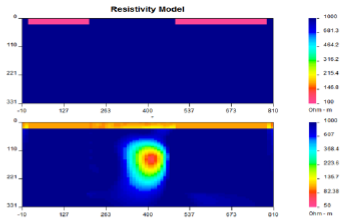
\includegraphics[width=0.5\columnwidth]{bAllWghtAct}
\caption{The reference model with an extended region of inactive cells is shown in the top panel. The recovered model from the subsequent inversion using both weighting and inactive cell constraints is presented in the bottom panel.}
\label{fig:bAllWghtAct}
\end{figure}